\newglossaryentry{airmass}{
name ={Airmass},
text={airmass},
description={Es el largo del camino de que le toma a los rayos de una cuerpo celeste atravesar la atm\'osfera. A medida que los rayos van penetrando la atm\'osfera estos se van atenuando por la absorci\'on y el proceso conocido como scattering. La cantidad de aire directamente perpendicular a la tierra se conoce como \textit{un airmass} y var\'ia con la elevaci\'on sobre el nivel del mar.\\
\begin{center}
\protect\fbox{\protect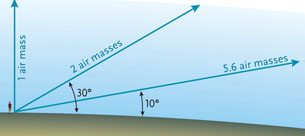
\includegraphics[scale=2.0]{images/airmasses}}
\captionof{figure}{Mientras m\'as cerca est\'e el objeto del horizonte, mayor ser\'a la cantidad de airmass por la que se observar\'a y mayor ser\'a  la distorci\'on sobre la imgen percibida del objeto. \textit{Reed, C. 2008; \url{https://www.skyandtelescope.com/astronomy-resources/transparency-and-atmospheric-extinction/}}}
\end{center}
}}

\newglossaryentry{kernel}{%
  name={Kernel },
  text={kernel},
  description={En el procesamiento de im\'agenes, un kernel corresponde a una matriz convolucional. Por lo general es usada para la modificaci\'on de im\'agenes o detecci\'on de bordes. Un ejemplo de kernel para este caso es el kernel PSF. \\En estad\'istica bayesiana, el kernel de una densidad de probabilidad es la forma de esta en la que se ha omitido todo tipo de factor que no es funci\'on de ninguna de las variables del dominio.  
  }
}

\newglossaryentry{psf}{%
  name={PSF},
  description={Corresponde a la respuesta instrumental a una fuente de luz puntual, cuya radiaci\'on debe atravesar la atm\'osfera terrestre y los lentes del telescopio. La distorsi\'on puede ser interpretada como la convoluci\'on de la imagen por un kernel.\\
\begin{center}
  \protect\fbox{\protect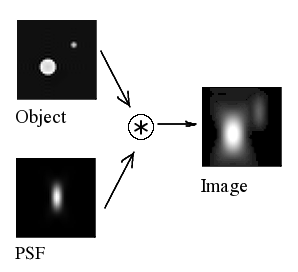
\includegraphics[scale=.5]{images/psf}}
  \captionof{figure}{Ejemplo de distorsi\'on de una fuente al aplicar un kernel de PSF espec\'ifico. El resultado se observa en el cuadro \textit{Image}. \textit{P. Huentelemu, 2016 \cite{huentelemu}}}
\end{center}   
}
}




%\begin{figure}[h]
%\centering
%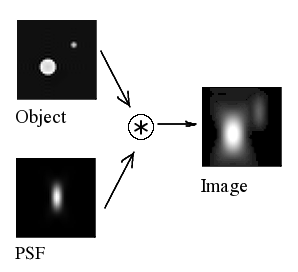
\includegraphics[scale=.5]{images/psf}
%\caption{Ejemplo de distorsi\'on de una fuente al aplicar un kernel de PSF espec\'ifico. El resultado se observa en el cuado \textit{Image}.}
%\label{fig:a1}
%\end{figure} 
